\begin{columns}
  \begin{column}{0.17\linewidth}
    
\includegraphics[width=0.5\linewidth]{fig/kth_cmyk.eps}
    \hfill
  \end{column}
  \hfill
  \begin{column}{0.64\linewidth}
    \begin{center}
      \Huge\bfseries
      Securely and Privately Verifiable Protests
    \end{center}
    \begin{center}
      \large
      Daniel Bosk <dbosk@kth.se>
      $\bullet$
      Sonja Buchegger
      $\bullet$
      Sébastien Gambs
    \end{center}
    \vspace{1.5em}
  \end{column}
  \hfill
  \begin{column}{0.17\linewidth}
    \hfill
    
\includegraphics[width=0.8\linewidth]{fig/uqam.pdf}
  \end{column}
\end{columns}

\includegraphics[width=\linewidth]{art/ProtestVerif.png}

\begin{columns}[t]

  \begin{column}{0.32\linewidth}

    \begin{redblock}{Verifying protest participation}
      \begin{itemize}
        \item Alice wants to show that many support her cause.
        \item Eve wants to show that few support Alice's cause.
        \item \color{red} Adversarial setting, requires verifiable results!
      \end{itemize}
    \end{redblock}

    \begin{figure}
      \centering
      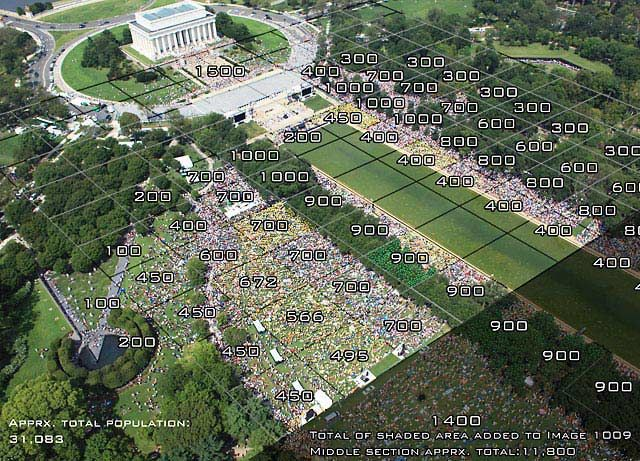
\includegraphics[width=0.9\linewidth]{fig/Jacobs-method.jpg}
      \caption{%
        Jacobs Method, currently most used method.
        Divide into regions, estimate density in each region, sum up.
        Image: popularmechanics.com
      }\label{JacobsMethod}
    \end{figure}

  \end{column}

  \begin{column}{0.32\linewidth}

    \begin{blueblock}{Requirements for verifiability}
      \begin{itemize}
        \item\label{EligibilityVerif} Eligibility: anyone can verify that each 
          participation proof provides temporal and spatial eligibility and that 
          it has not been counted before.

        \item\label{UniversalVerif} Universal verifiability: anyone can verify 
          that the result is according to the submitted participation proofs.

        \item\label{IndividualVerif} Individual verifiability: every participant 
          can verify that their participation proof is included in the global 
          count.
      \end{itemize}
    \end{blueblock}

    \begin{blueblock}{Requirements for privacy}
      \begin{itemize}
        \item The verifiability protocol should not increase the risk already 
          incurred by attending.
      \end{itemize}
    \end{blueblock}

  \end{column}

  \begin{column}{0.32\linewidth}

    \begin{greenblock}{Our approach}
      \begin{itemize}
        \item Provides a \emph{lower bound} of the participation count.
        \item Provides a verifiable participation count.
        \item Provides privacy based on anonymous credentials.
        \item The only added risk (over not using this) is if someone can use 
          your secret key.
        \item Requires only local connectivity during the protest.
      \end{itemize}
    \end{greenblock}

    \includegraphics[width=\linewidth]{art/ProtestVerif-UN.png}

  \end{column}

\end{columns}

\vspace{5em}

\begin{columns}[t]

  \begin{column}{0.32\linewidth}

    \begin{figure}
      \centering
      \begin{tikzpicture}[%
        -Latex,
        item/.style={rectangle,draw},
        edge from parent/.style={},
        ]
        \tikzset{%
          %grow'=left,%
          %level distance=5em%
        }
        \node[item] (proof) {Proof share}
        child {%
          node[item] (pid) {$pid$}
          child {%
            node[item] (cid) {$cid$}
            child {%
              node[item] (manifesto) {Manifesto}
            }
          }
        }
        child {%
          node[item] (wid) {$wid$}
        }
        child {%
          node[item] (ts) {$t_s$}
        }
        child {%
          node[item] (l) {$l$}
        }
        child {%
          node[item] (wsig) {$wsig$}
        }
        ;

        \path[every node/.style={font=\small}]
        (pid) edge node [anchor=south east] {$\in$} (proof)
        (wid) edge node [anchor=east] {$\in$} (proof)
        (ts) edge node [anchor=east] {$\in$} (proof)
        (l) edge node [anchor=west] {$\in$} (proof)
        (wsig) edge node [anchor=south west] {$\in$} (proof)
        ;

        \path[every node/.style={font=\small}]
        (manifesto) edge node [anchor=east] {$H(\cdot)$} (cid)
        (cid) edge node [anchor=east] {$PRF_{k_P}(\cdot)$} (pid)
        (pid) edge[bend right] node [anchor=north west] {$PRF_{k_W}(\cdot)$} (wid)
        % wsig
        (l) edge[bend right] (wsig)
        (ts) edge[bend right] (wsig)
        (wid) edge[bend right] node [anchor=north west] {$PRF_{k_W}(\cdot, \cdot, 
          \cdot)$} (wsig)
        ;

      \end{tikzpicture}
      \caption{%
        Structure of a proof share.
        The protester \(P\)'s identifier \(pid\) is computed using the protester's 
        key \(k_P\).
        The witness \(W\)'s identifier \(wid\) is computed using the witness's key 
        \(k_W\).
        \(t_s\) is a time interval and \(l\) is the coordinates of an area.
        The protest (cause) identifier \(cid\) is the hash value of the manifesto.
      }%
      \label{ProofShare}
    \end{figure}%

    \begin{figure}
      \centering
      \begin{minipage}{\linewidth}
        \begin{align*}
          O\to \text{all}\colon & \text{manifesto} \\
          P\colon & cid\gets H(\text{manifesto}), \\
          & pid\gets PRF_{k_P}(cid) \\
          P\to W\colon & pid \\
          W\leftrightarrow P\colon & \text{perform distance bounding} \\
          W\colon & wid\gets PRF_{k_W}(pid), \\
          & wsig\gets PRF_{k_W}(wid, t_s, l) \\
          W\to P\colon & (wid, t_s, l, wsig) \\[-1em]
          && \text{during protest} \\ \hline && \text{after protest} \\[-1em]
          W\to S\colon & H(pid, wid, t_s, l, wsig) \\
          P\to S\colon & H(pid, wid, t_s, l, wsig) \\
          W\to S\colon & (pid, wid, t_s, l, wsig),\\
            & NIZK( wid = PRF_{k_W}(pid), \\
            & wsig = PRF_{k_W}(wid, t_s, l), \\
            & \exists sign(k_W)) \\
          P\to S\colon & (pid, wid, t_s, l, wsig),\\
          & NIZK(pid = PRF_{k_P}(cid), \exists sign(k_P))
        \end{align*}
      \end{minipage}
      \caption{%
        An overview of message exchanges.
        The organizer \(O\) broadcasts the manifesto.
        \(P\), \(W\) and their computations are as in \cref{fig:ProofFig}.
        Finally, both \(P\) and \(W\) submits the proof share to the storage \(S\).
      }%
      \label{Protocol}
    \end{figure}

    \printbibliography[heading=none]

  \end{column}

  \hfill

  \begin{column}{0.32\linewidth}

    \begin{blackblock}{Technically, during protest}
      \begin{itemize}
        \item The organizer publishes the protest's manifesto.
        \item Each protester reads it, approves it, computes a protest (cause) 
          identifier (\(cid\)) to designate which protest they participate in.
        \item Each protester computes a personal identifier (\(pid\)), 
          unlinkable between protests,
        \item Each protester acts as witness (unlinkable between protesters) for 
          other protesters by creating participation-proof shares.
        \item Proof shares vouches for temporal and spatial eligibility.
        \item A threshold-based number of valid shares is a valid proof.
      \end{itemize}
    \end{blackblock}

    \begin{blackblock}{Technically, after the protest}
      \begin{itemize}
        \item Proof shares are committed to a blockchain as soon as possible.
        \item \Ac{NIZK} proofs of correctness of \(PRF\) computations and 
          validity of keys are submitted whenever convenient.
        \item Anyone can verify the proofs: eligibility, universal and 
          individual verifiability.
        \item Must be done for all shares and their \ac{NIZK} proofs.
        \item Count all \(pid\)s with valid proofs.
      \end{itemize}
    \end{blackblock}

  \end{column}

  \hfill

  \begin{column}{0.32\linewidth}

    \begin{block}{More info}
      \begin{center}
        \includegraphics[width=0.4\linewidth]{fig/qr.eps}
      \end{center}
    \end{block}

  \end{column}

\end{columns}

\flushright
Special thanks to xkcd.com who, over many years, has inspired the stylistic 
presentation of this poster.
